\documentclass[letterpaper,12pt]{article}
\usepackage[letterpaper]{geometry}

\usepackage{amsmath,amsthm,enumitem,cleveref}
\setlist{itemsep=0pt}

\usepackage{tikz,tikz-cd,adjustbox}
\tikzcdset{
	arrow style=math font
}

\usepackage[bitstream-charter]{mathdesign}
\usepackage[T1]{fontenc}
\usepackage{relsize}

\newcommand{\N}{\mathbb{N}}
\newcommand{\F}{\mathbb{F}}
\newcommand{\R}{\mathbb{R}}

\newcommand{\from}{\leftarrow}
\newcommand{\iso}{\cong}

\newcommand{\after}{\circ}
\newcommand{\union}{\cup}
\newcommand{\dunion}{\sqcup}

\newcommand{\cat}[1]{\mathbf{#1}}
\newcommand{\dual}[1]{#1^{\mathrm{op}}}
\newcommand{\Cat}{\cat{Cat}}
\newcommand{\Set}{\cat{Set}}
\newcommand{\Vect}{\cat{Vect}}
\newcommand{\VectFin}{\Vect_{\mathrm{fin}}}

\renewcommand{\star}[1]{#1^{*}}
\newcommand{\pair}[2]{({#1},{#2})}
\newcommand{\copair}[2]{[{#1},{#2}]}

\newcommand{\textdefn}{\textbf}

\theoremstyle{definition}
\newtheorem{defn}[equation]{Definition}
\newtheorem{exmp}[equation]{Example}

\theoremstyle{plain}
\newtheorem{propy}[equation]{Property}
\newtheorem{prop}[equation]{Proposition}
\newtheorem{thm}[equation]{Theorem}
\newtheorem{cor}[equation]{Corollary}

% numbering
\numberwithin{equation}{section}

% meta
\title{Abstract Nonsense\\{\smaller A Glance at Category Theory}}
\author{John Peloquin}
%\date{}

\begin{document}
% title
\maketitle

\section*{Introduction}
In this paper we take a quick glance at category theory. More specifically, we review the basic vocabulary and concepts of categories, functors, naturality, universality, and duality along with a number of simple examples.

Why category theory? An analogy might help motivate our study. When I was a kid, I was obsessed with traffic cones. My parents would sometimes steal them for me, from parking lots or construction sites, and my love for the cones made me look past this unethical behavior. I would categorize and compare the cones in various ways---by size, shape, color, pattern, etc.---and derive great pleasure and insight from this.

Category theory allows us to similarly gain insight into important relationships between mathematical objects. It's a sort of universal mathematical language which tends to reveal connections between seemingly unrelated subjects, like logic and geometry. It's also highly abstract---as in the title of this paper, it's sometimes jokingly referred to as ``abstract nonsense''---but it yields elegant and powerful results which are useful in many areas of mathematics and beyond.

We won't look deeply into the theory in this paper, but we'll try to get an intuition for the basics from our glance. Those who prefer noises and moving pictures to prose should note that some of this material is based on my video series available at~\cite{peloquin}.

% categories
\section{Categories}
So, what's a category? It consists of two types of things:
\begin{itemize}
\item \textdefn{Objects:} \(A,B,C,\ldots\)
\item \textdefn{Arrows:} \(f,g,h,\ldots\)
\end{itemize}
Each arrow has a unique \textdefn{domain} (or \textdefn{source}) object and a unique \textdefn{codomain} (or \textdefn{target}) object. We write \(f:A\to B\) or
\begin{equation*}
\begin{tikzcd}
A \ar[r,"f"] & B
\end{tikzcd}
\end{equation*}
(read ``\(f\) from~\(A\) to~\(B\)'') to indicate that \(f\)~is an arrow with domain~\(A\) and codomain~\(B\). Importantly, in this definition we won't say \emph{what} the objects and arrows are; we'll only specify the properties they must satisfy to constitute a category. This is what makes the definition abstract.

First, for arrows \(f:A\to B\) and \(g:B\to C\), there's a \textdefn{composite} arrow \(g\after f:A\to C\) making this diagram ``commute'':
\begin{equation}
\begin{tikzcd}
A \ar[rd,dashed, "g\after f"'] \ar[r,"f"] & B \ar[d,"g"] \\
  & C
\end{tikzcd}
\label{cd:composite}
\end{equation}
The composite \(g\after f\) (read ``\(g\) after \(f\)'') represents the result of first applying \(f\) and then applying \(g\). The diagram~\eqref{cd:composite} is said to commute because, starting at~\(A\), you can either go across to~\(B\) along~\(f\) and then down to~\(C\) along~\(g\), or you can go diagonally from \(A\) to~\(C\) along \(g\after f\) and get the same result. Commutative diagrams like~\eqref{cd:composite} are used frequently in category theory because they provide a way to visualize what's happening in a category.

Second, every object~\(A\) has an \textdefn{identity} arrow \(1_A:A\to A\). We don't usually draw identity arrows in diagrams.

Third, the law of composition for arrows needs to satisfy two properties:
\begin{itemize}
\item \textdefn{Associativity:}
\[h\after(g\after f)=(h\after g)\after f\]
for all \(f:A\to B\), \(g:B\to C\), and \(h:C\to D\).
\item \textdefn{Unity:}
\[f\after 1_A=f=1_B\after f\]
for all \(f:A\to B\).
\end{itemize}
Associativity allows us to drop the parentheses when composing three or more arrows---for example, we can just write \(h\after g\after f\) for the arrow above. Unity says that the identity arrows don't do anything. But they're still useful! Just like the number~\(0\) is useful for addition and the number~\(1\) is useful for multiplication.

These properties seem somewhat technical when written out, but they're actually very natural and satisfied in many situations. In summary, we have a definition:
\begin{defn}
A \textdefn{category} is a collection of objects, and arrows between those objects, with a law of composition for arrows that's associative and unital.
\end{defn}

\subsection{Examples}
We now look at some examples of categories.
\begin{exmp}
In the category~\(\Set\), sets are the objects and functions are the arrows.\footnote{We don't define a function to be a set of ordered pairs, but treat it as a primitive, undefined concept which is intuitively understood.} For instance the set
\[\N=\{\,0,1,2,\ldots\,\}\]
of natural numbers is an object in~\(\Set\), and the successor function \(\sigma:\N\to\N\) given by \(\sigma(n)=n+1\) is an arrow in~\(\Set\). The function \(\tau:\N\to\{\,1,2,\ldots\,\}\) given by \(\tau(n)=n+1\) is a \emph{different} arrow, because it has a different codomain.

Every set has an identity function which maps elements to themselves, and function composition is associative and unital, so \(\Set\)~really is a category.
\end{exmp}

\noindent There are many categories in which the objects are ``structured'' sets and the arrows are ``structure-preserving'' functions. In these categories, composites and identities are defined as in~\(\Set\). Here's an example:
\begin{exmp}
In the category~\(\Vect_{\F}\), vector spaces over the field~\(\F\) are the objects and linear maps over~\(\F\) are the arrows.
\end{exmp}

\noindent Importantly, the objects in a category need not have elements, and the arrows need not be functions. A big part of adjusting to the category-theoretic viewpoint is learning to live without such elements.

Recall that a \textdefn{preorder} is a pair \((P,{\le})\) where \(P\)~is a set and \({\le}\)~is a binary relation on~\(P\) which is reflexive and transitive.
\begin{exmp}
Every preorder can be viewed as a category in which the objects are the elements of the preorder and there's a (unique) arrow \(a\to b\) if and only if \(a\le b\). The identity arrows \(a\to a\) exist by reflexivity. The composite of the arrows \(a\to b\) and \(b\to c\) is the arrow \(a\to c\) which exists by transitivity. A moment's thought shows that composition is associative and unital.
\end{exmp}
\noindent This example also illustrates that when you define a new category, you don't need to give it a name and break a champagne bottle. (However you may want to drink some champagne, especially if you're a raging alcoholic.)

Sometimes it's useful to treat arrows in one category as objects in another. Here's an example like that to expand your mind:
\begin{exmp}
For a category~\(\cat{C}\) and fixed object \(C\) in~\(\cat{C}\), consider the category of ``arrows over~\(C\)'' with the following data:
\begin{itemize}
\item \textbf{Objects:} arrows in~\(\cat{C}\) of the form \(A\to C\)
\item \textbf{Arrows:} an arrow from \(f:A\to C\) to \(g:B\to C\) is an arrow \(h:A\to B\) in~\(\cat{C}\) making this diagram commute in~\(\cat{C}\):\footnote{Technically we take the arrow to be the triple \((h,f,g)\) in order to keep track of the domain~\(f\) and codomain~\(g\), so that \((h,f,g):f\to g\). Recall that an arrow in a category must have a \emph{unique} domain and a \emph{unique} codomain.}
\begin{equation*}
\begin{tikzcd}[column sep=small]
A \ar[rd, "f"'] \ar[rr, "h"] && B \ar[ld, "g"]\\
  & C &
\end{tikzcd}
\end{equation*}
\end{itemize}
Composites and identities are inherited from~\(\cat{C}\).
\label{exmp:slicecat}
\end{exmp}

\subsection{Isomorphisms}
Using categories, we can define an important general notion:
\begin{defn}
In a category~\(\cat{C}\), an arrow \(f:A\to B\) is an \textdefn{isomorphism} if there's an arrow \(g:B\to A\) in~\(\cat{C}\) with
\[g\after f=1_A\qquad f\after g=1_B\]
In this case, we say that \(f\) and~\(g\) are \textdefn{inverse}. We also say that \(A\) and~\(B\) are \textdefn{isomorphic} and write \(A\iso B\).
\end{defn}
\noindent Note that this definition is totally abstract as it applies in \emph{any} category. Intuitively, isomorphic objects have identical structure.

\begin{exmp}
In~\(\Set\), the isomorphisms are the bijections, so sets are isomorphic if and only if they have the same size.
\end{exmp}

% functors
\section{Functors}
Categories themselves have internal structure which can be preserved by mappings. Consider the mapping~\(P\) which sends a set~\(A\) to its \textdefn{powerset}
\begin{equation}
P(A)=\{\,X\mid X\subseteq A\,\}
\label{eq:powersetset}
\end{equation}
This mapping acts on objects in~\(\Set\), but we can extend it to act on arrows also. For a function \(f:A\to B\), we define the function \(P(f):P(A)\to P(B)\) by
\begin{equation}
P(f)(X)=\{\,f(x)\mid x\in X\,\}
\label{eq:powersetfunc}
\end{equation}
This definition works, since if \(x\in X\subseteq A\), then \(f(x)\in B\), so \(P(f)(X)\subseteq B\). The mapping~\(P\) ``lifts'' the action of~\(f\) from elements of~\(A\) to subsets of~\(A\), as seen in \Cref{fig:powerset}.
\begin{figure}[h]
\centering
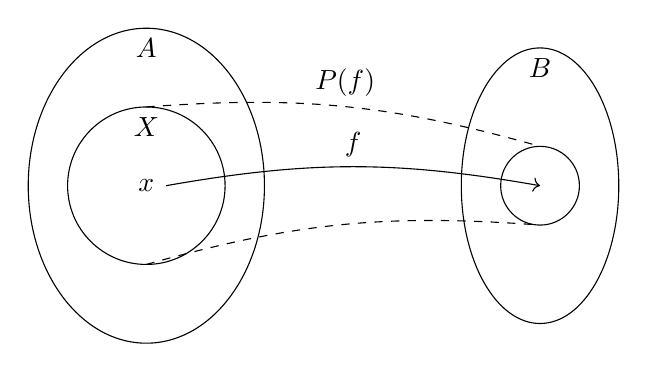
\begin{tikzpicture}
  \draw (0,0) ellipse (1.5 and 2);
  \node at (0,1.75) {$A$};
  
  \draw (0,0) circle (1);
  \node at (0,0.75) {$X$};
  \node at (0,0) {$x$};
  
  \draw (5,0) ellipse (1 and 1.75);
  \node at (5,1.5) {$B$};
  \draw (5,0) circle (0.5);
  
  \draw[->, bend left=10] (0.25,0) to node[midway, above] {$f$} (5,0);
  \draw[-, dashed, bend left=10] (0,1) to node[midway, above] {$P(f)$} (5,0.5);
  \draw[-, dashed, bend left=10] (0,-1) to (5,-0.5);
\end{tikzpicture}
\caption{It kinda looks like eggs.}
\label{fig:powerset}
\end{figure}

Importantly, the mapping preserves composites and identities as it moves us up the cumulative hierarchy in~\(\Set\). If \(g:B\to C\) is another function, then
\[P(g\after f)=P(g)\after P(f)\]
and
\[P(1_A)=1_{P(A)}\]
as you can verify from the definitions. Mappings like this which preserve categorical structure have a name:
\begin{defn}
For categories \(\cat{C}\) and~\(\cat{D}\), a \textdefn{functor} \(F:\cat{C}\to\cat{D}\) is a mapping which
\begin{enumerate}[label=(\roman*)]
\item maps objects in~\(\cat{C}\) to objects in~\(\cat{D}\)
\item maps arrows \(A\to B\) in~\(\cat{C}\) to arrows \(F(A)\to F(B)\) in~\(\cat{D}\)
\item preserves composites:
\[F(g\after f)=F(g)\after F(f)\]
for all arrows \(f:A\to B\) and \(g:B\to C\) in~\(\cat{C}\).
\item preserves identities:
\[F(1_A)=1_{F(A)}\]
for all objects \(A\) in~\(\cat{C}\).
\end{enumerate}
\end{defn}
\noindent It's easier to understand this definition using diagrams. For every commutative triangle in the category~\(\cat{C}\), the functor \(F:\cat{C}\to\cat{D}\) creates a corresponding commutative triangle in~\(\cat{D}\):
\begin{equation}
\begin{tikzcd}[column sep=small]
& \cat{C} \ar[rrrr, Rightarrow, shorten=1em, bend left=10, "F"] &&&& \cat{D} & \\
A \ar[rrd, "g\after f"'] \ar[rr,"f"] && B \ar[d,"g"] && F(A) \ar[rrd, "F(g\after f)"'] \ar[rr,"F(f)"] && F(B) \ar[d,"F(g)"] \\
  && C && && F(C)
\end{tikzcd}
\end{equation}
So \(F\)~creates a ``diagram of shape~\(\cat{C}\)'' in~\(\cat{D}\). However, in general that diagram may be ``deformed''---for example there's nothing to prevent \(F(f)=F(g)\) in~\(\cat{D}\) even if \(f\ne g\) in~\(\cat{C}\).

\subsection{Examples}
We've already seen one example of a functor:
\begin{exmp}
The mapping \(P:\Set\to\Set\) defined in \eqref{eq:powersetset} and~\eqref{eq:powersetfunc} above is the \textdefn{powerset functor}.
\end{exmp}

\noindent Let's look at a few more. In categories of structured sets, just as in life, sometimes we want to forget:
\begin{exmp}
The \textdefn{forgetful functor} \(U:\Vect_{\F}\to\Set\) maps each vector space to its underlying set, and each linear map to its underlying function. Here \(U\)~``forgets'' all about addition and scalar multiplication and linearity, but it preserves composites and identities.
\end{exmp}

\noindent Sometimes we see familiar faces:
\begin{exmp}
If \((P,\le)\) and~\((Q,\preccurlyeq)\) are preorders, then a functor \(F:P\to Q\) is precisely a \textdefn{monotone function}, which means that \(a\le b\) implies \(F(a)\preccurlyeq F(b)\).
\end{exmp}

\noindent Every category~\(\cat{C}\) has an \textdefn{identity functor} \(1_{\cat{C}}:\cat{C}\to\cat{C}\) which maps objects and arrows to themselves. If \(F:\cat{C}\to\cat{D}\) and \(G:\cat{D}\to\cat{E}\) are functors, then the \textdefn{composite functor} \(G\after F:\cat{C}\to\cat{E}\) is defined in the obvious way. (It behooves you to check that these really are functors.) Functor composition is associative and unital, which should make you suspicious that something's afoot. Indeed, we have another example of a category:
\begin{exmp}
In the category~\(\Cat\), categories are the objects and functors are the arrows.
\end{exmp}
\noindent If you've studied any set theory, you're probably getting uncomfortable. Is \(\cat{Cat}\) an object in~\(\cat{Cat}\)? Would that be a problem? Didn't Bertrand Russell make a good living disparaging Christians and finding paradoxes with stuff like this? Well, maybe, but we're going to ignore ``foundational'' questions of this sort because they're irrelevant to our glance at category theory. I encourage the anxious reader to get a Xanax\texttrademark\ prescription.

% natural transformations
\section{Natural transformations}
In categories, sometimes arrows don't depend in any essential way on the particular objects they relate. Such arrows are called ``natural''. As an example in~\(\Set\), recall that the \textdefn{cartesian product} of sets \(A\) and~\(B\) is defined by
\begin{equation}
A\times B=\{\,(x,y)\mid x\in A\text{ and }y\in B\,\}
\label{eq:cartesianprod}
\end{equation}
There's a ``swap'' function
\begin{equation*}
\begin{tikzcd}
A\times B \ar[r,"s_{AB}"] & B\times A
\end{tikzcd}
\end{equation*}
defined by \(s_{AB}(x,y)=(y,x)\). For any other sets \(C\) and~\(D\) there's also a corresponding swap function
\begin{equation*}
\begin{tikzcd}
C\times D \ar[r,"s_{CD}"] & D\times C
\end{tikzcd}
\end{equation*}
Now intuitively, the swap function doesn't depend in an essential way on the particular sets it swaps, since it's defined ``in the same way'' for any pair of sets. But how can we make this intuition precise? One way is using the perspective of category theory.

For any functions \(f:A\to C\) and \(g:B\to D\), this diagram commutes:
\begin{equation}
\begin{tikzcd}
A\times B \ar[d, "f\times g"'] \ar[r, "s_{AB}"] & B\times A \ar[d, "g\times f"] \\
C\times D \ar[r, "s_{CD}"'] & D\times C
\end{tikzcd}
\label{cd:swap}
\end{equation}
Here \(f\times g\)~is defined by
\[(f\times g)(x,y)=(f(x),g(y))\]
and similarly for~\(g\times f\). We have
\begin{align*}
[s_{CD}\after(f\times g)](x,y)&=s_{CD}(f(x),g(y))\\
	&=(g(y),f(x))\\
	&=(g\times f)(y,x)\\
	&=[(g\times f)\after s_{AB}](x,y)
\end{align*}
so
\[s_{CD}\after(f\times g)=(g\times f)\after s_{AB}\]
which is precisely commutativity of the diagram~\eqref{cd:swap}.

Commutativity of the diagram~\eqref{cd:swap} tells us that no matter how we ``transform'' the input sets \(A\) and~\(B\) to obtain the output sets \(C\) and~\(D\), we can \emph{either} first transform the input sets and then swap the output sets \emph{or} first swap the input sets and then transform them in the swapped order---we get the same result either way. So the swap function must behave in the same way for any pair of sets.

There's actually a functor lurking here, which involves a new type of category:
\begin{defn}
For categories \(\cat{C}\) and~\(\cat{D}\), the \textdefn{product category} \(\cat{C}\times\cat{D}\) consists of
\begin{itemize}
\item \textbf{Objects:} pairs \((C,D)\) of objects with \(C\) in~\(\cat{C}\) and \(D\) in~\(\cat{D}\)
\item \textbf{Arrows:} pairs \((f,g)\) of arrows with \(f\) in~\(\cat{C}\) and \(g\) in~\(\cat{D}\)
\end{itemize}
Composites and identities are defined componentwise. Note this is like a ``cartesian product'' in~\(\Cat\), and it can be defined for more than two categories. The product
\[\underbrace{\cat{C}\times\cdots\times\cat{C}}_{n\text{ copies}}\]
is sometimes written~\(\cat{C}^n\).
\label{defn:productcat}
\end{defn}
\noindent We can define a product functor \(F:\Set^2\to\Set\) by
\[F(A,B)=A\times B\qquad F(f,g)=f\times g\]
We can also define a ``swapped'' product functor \(G:\Set^2\to\Set\) by
\[G(A,B)=B\times A\qquad G(f,g)=g\times f\]
(I don't need to remind you to check that these really are functors, because you're a diligent and virtuous person.) In terms of these functors, diagram~\eqref{cd:swap} becomes
\begin{equation}
\begin{tikzcd}
F(A,B) \ar[d, "{F(f,g)}"'] \ar[r, "s_{AB}"] & G(A,B) \ar[d, "{G(f,g)}"] \\
F(C,D) \ar[r, "s_{CD}"'] & G(C,D)
\end{tikzcd}
\label{cd:swapfunc}
\end{equation}
So we see that swapping is a family of functions between the image objects of the functors \(F\) and~\(G\) which respects the image arrows of \(F\) and~\(G\). In fact, swapping can be seen as a type of arrow \(s:F\to G\) between the functors:
\begin{defn}
For categories \(\cat{C}\) and~\(\cat{D}\) and functors \(F:\cat{C}\to\cat{D}\) and \(G:\cat{C}\to\cat{D}\), a \textdefn{natural transformation} \(\nu:F\to G\) is a family of arrows in~\(\cat{D}\)
\[\nu_C:F(C)\to G(C)\]
for all objects \(C\) in~\(\cat{C}\), such that for all arrows \(f:A\to B\) in~\(\cat{C}\) this diagram commutes in~\(\cat{D}\):
\begin{equation}
\begin{tikzcd}
F(A) \ar[d, "F(f)"'] \ar[r, "\nu_A"] & G(A) \ar[d, "G(f)"] \\
F(B) \ar[r, "\nu_B"'] & G(B)
\end{tikzcd}
\end{equation}
The arrow \(\nu_C\)~is the \textdefn{component} of~\(\nu\) at~\(C\). By abuse of language, sometimes \(\nu_C\)~is called a natural transformation or is said to be ``natural in~\(C\)''.
\end{defn}
\noindent We can visualize a natural transformation as seen in \Cref{fig:nat}. Notice how it creates a ``cylinder'' or ``prism'' between the image diagrams of the functors, each face of which is a commutative diagram.
\begin{figure}[h]
\centering
\adjustbox{scale=0.75}{
\begin{tikzcd}[sep=huge]
A \ar[r, "f"] \ar[rd, "g\after f"' name=gf] & B \ar[d, "g" name=g] & & \\
 & C & & \\
 & & G(A) \ar[r, "G(f)" name=Gf] \ar[rd, "G(g\after f)"'] & G(B) \ar[d, "G(g)"] \\
 & & & G(C) \\
F(A) \ar[r, "F(f)" name=Ff] \ar[rd, "F(g\after f)"'] \ar[rruu, dashed, bend left, "\nu_A"] & F(B) \ar[d, "F(g)"] \ar[rruu, dashed, bend left, end anchor=south west, crossing over, "\nu_B"] & & \\
 & F(C) \ar[rruu, dashed, bend left, start anchor=north east, "\nu_C"] & &
 \ar[from=gf, to=Ff, Rightarrow, shorten <=2em, shorten >=5em, bend right=20, "F"{', inner sep=1.25em, yshift=3em}]
 \ar[from=g, to=Gf, Rightarrow, shorten=3em, bend left=10, "G" inner sep=0.75em]
\end{tikzcd}
}
\caption{It feels natural.}
\label{fig:nat}
\end{figure}
\goodbreak
A natural transformation really is an arrow, in a certain type of category:
\begin{defn}
For categories \(\cat{C}\) and~\(\cat{D}\), the \textdefn{functor category} \(\cat{D}^\cat{C}\) consists of
\begin{itemize}
\item \textbf{Objects:} functors \(\cat{C}\to\cat{D}\)
\item \textbf{Arrows:} natural transformations between those functors
\end{itemize}
Composites and identities are defined componentwise.
\end{defn}
\noindent We won't talk more about functor categories in this paper, but they sure are fine lookin' specimens which make me feel tingly inside.

\subsection{Examples}
We've already seen a simple example of naturality:
\begin{exmp}
Swapping sets in a cartesian product~\eqref{eq:cartesianprod} is a natural transformation. In fact since swapping is also invertible, it's a \textdefn{natural isomorphism}---that is, a natural transformation whose components are isomorphisms:
\[A\times B\iso B\times A\]
This shows that the cartesian product operation is commutative up to isomorphism---a fact that has nothing to do with the objects \(A\) and~\(B\) and everything to do with the product operation itself. The concept of naturality allows us to elegantly capture this.
\end{exmp}

\begin{exmp}
A similar one is the associativity isomorphism
\[(A\times B)\times C\iso A\times(B\times C)\]
which is natural in the sets \(A\), \(B\), and~\(C\). (You should verify this by exhibiting a natural isomorphism between functors \(\Set^3\to\Set\).)
\end{exmp}

\noindent There are countless other examples like this in mathematics. Rather than looking at more, we turn to another important concept.

% universal properties
\section{Universal properties}
A universal property characterizes an object in a category, in an essentially unique way, in terms of its relation to other objects through arrows. This stands in contrast to characterizations that refer to intrinsic ``implementation details'' of an object which are irrelevant from a category-theoretic perspective.

By doing this, a universal property abstracts away potentially complicated or messy details of a particular construction, leading to more elegant results. It also allows us to avoid repeating the same proofs over and over again in different situations. Once we know that an object in a category is universal, anything that follows from the universal property is known to be true of that object.

The best way to learn about universal properties is to look at many examples and see what they have in common. We'll look at a few choice examples in this section.

\subsection{Products}
To start, recall from~\eqref{eq:cartesianprod} the cartesian product  of sets \(A\) and~\(B\) in~\(\Set\):
\[A\times B=\{\,(x,y)\mid x\in A\text{ and }y\in B\,\}\]
There are many things we could say about this product. As an example, we could talk about the way we're actually defining the ordered pairs using sets. Maybe we're using the Kuratowski pair
\begin{equation}
(x,y)=\{\{x\},\{x,y\}\}
\label{eq:kuratowskipair}
\end{equation}
Or maybe we're hot for the Wiener pair
\begin{equation}
(x,y)=\{\{\{x\},\varnothing\},\{\{y\}\}\}
\label{eq:wienerpair}
\end{equation}
From a set-theoretic perspective, both \eqref{eq:kuratowskipair} and~\eqref{eq:wienerpair} would be reasonable choices since they satisfy the required property of an ordered pair:
\[(x,y)=(x',y')\quad\iff\quad x=x'\text{ and }y=y'\]
From a category-theoretic perspective, however, we don't really care that the product consists of ordered pairs, let alone which type. Instead we care about something more abstract:
\begin{propy}
The cartesian product \(A\times B\) allows us to freely translate between a pair of functions \(X\to A\) and \(X\to B\) and a single function \(X\to A\times B\).
\label{propy:cartesianprod}
\end{propy}
\noindent This property completely characterizes the product---from it we can derive anything we really need, without relying on intrinsic implementation details. To see how this works, first note that there are \textdefn{projection} functions
\begin{equation}
\begin{tikzcd}
A & \ar[l,"p_1"'] A\times B \ar[r,"p_2"] & B
\end{tikzcd}
\label{cd:cartesianprod}
\end{equation}
defined by
\[p_1(x,y)=x\qquad p_2(x,y)=y\]
For any function \(p:X\to A\times B\), this diagram commutes:
\begin{equation}
\begin{tikzcd}
 & X \ar[ld,dashed,bend right,"p_1\after p"'] \ar[d, "p"] \ar[rd,dashed,bend left,"p_2\after p"] & \\
A & \ar[l,"p_1"'] A\times B \ar[r,"p_2"] & B
\end{tikzcd}
\label{cd:cartesianprodproj}
\end{equation}
So from a single function \(X\to A\times B\) we obtain a pair of functions \(X\to A\) and \(X\to B\).

Conversely, for \emph{any} functions \(f:X\to A\) and \(g:X\to B\), we can define the \textdefn{pair} function \((f,g):X\to A\times B\) by
\[(f,g)(x)=(f(x),g(x))\]
which is unique making this diagram commute:
\begin{equation}
\begin{tikzcd}
 & X \ar[ld,bend right,"f"'] \ar[d,dashed,"{(f,g)}"] \ar[rd,bend left,"g"] & \\
A & \ar[l,"p_1"'] A\times B \ar[r,"p_2"] & B
\end{tikzcd}
\label{cd:cartesianprodpair}
\end{equation}
So from a pair of functions \(X\to A\) and \(X\to B\) we obtain a single function \(X\to A\times B\). Moreover, it follows from \eqref{cd:cartesianprodproj} and~\eqref{cd:cartesianprodpair} that these operations are mutually inverse, since
\[p=(p_1\after p,p_2\after p)\]
and
\[f=p_1\after(f,g)\qquad g=p_2\after(f,g)\]
This establishes \Cref{propy:cartesianprod} and shows that the cartesian product~\eqref{cd:cartesianprod} is ``universal'' as a set with a pair of functions into \(A\) and~\(B\)---indeed, \emph{any} pair of functions from a set into \(A\) and~\(B\) can be obtained through~\eqref{cd:cartesianprod} in a unique way. We can use this as the basis of an abstract definition of a product:
\begin{defn}
In a category, a \textdefn{product} of objects \(A\) and~\(B\) is an object~\(P\) and pair of arrows
\begin{equation}
\begin{tikzcd}
A & \ar[l,"p_1"'] P \ar[r,"p_2"] & B
\end{tikzcd}
\label{cd:product}
\end{equation}
such that for any pair of arrows
\begin{equation*}
\begin{tikzcd}
A & \ar[l,"f"'] X \ar[r,"g"] & B
\end{tikzcd}
\end{equation*}
there's a unique arrow \(p:X\to P\) making this diagram commute:
\begin{equation}
\begin{tikzcd}
 & X \ar[ld,bend right,"f"'] \ar[d,dashed,"p"] \ar[rd,bend left,"g"] & \\
A & \ar[l,"p_1"'] P \ar[r,"p_2"] & B
\end{tikzcd}
\label{cd:productump}
\end{equation}
The arrows \(p_1\) and~\(p_2\) are called \textdefn{projections}. The arrow \(p\)~is called a \textdefn{pair} and may be denoted \(p=\pair{f}{g}\). The object~\(P\) may be denoted \(A\times B\).
\end{defn}
\noindent A few remarks about this definition. First, it really is abstract! It applies in \emph{any} category, even one where the objects don't have elements. Second, it defines \emph{a} product of objects \(A\) and~\(B\), not \emph{the} product---we don't know that a product exists, and even if one exists it need not be unique. We'll talk more about uniqueness in a bit. Third, a product consists of the whole diagram~\eqref{cd:product}, not just the object~\(P\), although we often abuse language and say ``product~\(P\)''. Fourth, diagram~\eqref{cd:productump} exhibits a universal property---a product of \(A\) and~\(B\) is universal as an object with a pair of arrows into \(A\) and~\(B\), in the sense that \emph{any} pair of arrows from an object into \(A\) and~\(B\) can be obtained through the product in a unique way.

Here's an analogy that might help you understand all this. When I was a kid, my dad had a universal remote for the devices in our living room. It had hundreds of buttons and was almost impossible for anyone else to use, but it let him do multiple things at once---like look around for porn on the TV while recording Filipino stick fighting videos on the VCR. The point is that the functions of all the device remotes were obtained through the universal remote in a certain way, and in this sense it satisfied a universal property similar to that of a product~\eqref{cd:product}.

We've now seen some examples of products:
\begin{exmp}
In~\(\Set\), a cartesian product~\eqref{cd:cartesianprod} is a product.
\end{exmp}
\begin{exmp}
In~\(\Cat\), a product category (see \Cref{defn:productcat}) is also a product, by essentially the same reasoning.
\end{exmp}
\noindent Here's another cute example to think through:
\begin{exmp}
In a preorder, a product is precisely a \textdefn{greatest lower bound} (or \textdefn{infimum} or \textdefn{meet}). Look at the definition!
\end{exmp}

\subsection{Uniqueness}
Recall that I said some stuff earlier about universal properties characterizing objects ``essentially uniquely'' and giving us what we ``really need''. It sounds like new age garbage but it's also true. Rather than proving this for products directly, we'll start with a simpler universal object:
\begin{defn}
In a category, an object~\(T\) is \textdefn{terminal} if for every object \(C\) there's a unique arrow \(C\to T\).
\end{defn}
\noindent Here's the word:
\begin{prop}
Terminal objects are unique up to unique isomorphism. More precisely, if \(T\) and~\(T'\) are terminal objects in a category, then there's a unique isomorphism \(T\to T'\).\label{prop:terminalunique}
\end{prop}
\begin{proof}
There's a unique arrow \(f:T\to T'\) since \(T'\)~is terminal. There's also a unique arrow \(g:T'\to T\) since \(T\)~is terminal. Now we have the arrows \(g\after f:T\to T\) and \(1_T:T\to T\), so \(g\after f=1_T\) since \(T\)~is terminal. Similarly \(f\after g=1_{T'}\) since \(T'\)~is terminal. So \(f\) and~\(g\) are inverse isomorphisms.
\end{proof}
\noindent This result is interesting only to the extent that a terminal object is interesting, and a terminal object is interesting only to the extent that its ambient category is interesting. Consider:
\begin{exmp}
In~\(\Set\), the terminal objects are the singletons. Clearly, singletons have the same size.
\end{exmp}
\begin{exmp}
In a preorder, a terminal object is precisely a \textdefn{greatest} (or \textdefn{maximum}) element. Any two greatest elements are less than or equal to each other.
\end{exmp}

\begin{exmp}
For a category~\(\cat{C}\) and fixed objects \(A\) and~\(B\) in~\(\cat{C}\), construct the category of ``pairs of arrows from an object into \(A\) and~\(B\)'':
\begin{itemize}
\item \textbf{Objects:} diagrams in~\(\cat{C}\) of the form
\begin{equation*}
\begin{tikzcd}
A & \ar[l] X \ar[r] & B
\end{tikzcd}
\end{equation*}
\item \textbf{Arrows:} an arrow from \(A\from X\to B\) to \(A\from Y\to B\) is an arrow \(X\to Y\) in~\(\cat{C}\) making this diagram commute in~\(\cat{C}\):\footnote{Technically an arrow is a triple, as in \Cref{exmp:slicecat}.}
\begin{equation*}
\begin{tikzcd}
 & X \ar[ld,bend right] \ar[d] \ar[rd,bend left] & \\
A & \ar[l] Y \ar[r] & B
\end{tikzcd}
\end{equation*}
\end{itemize}
Composites and identities are inherited from~\(\cat{C}\). A terminal object in this category is precisely a product of \(A\) and~\(B\) in~\(\cat{C}\), as you should verify with excitement!
\label{exmp:productterminal}
\end{exmp}

\noindent From this we obtain uniqueness of products:
\begin{cor}
Products are unique up to unique isomorphism. More precisely, if \(A\) and~\(B\) are objects in a category and
\begin{equation*}
\begin{tikzcd}
A & \ar[l,"p_1"'] P \ar[r, "p_2"] & B
\end{tikzcd}
\end{equation*}
and
\begin{equation*}
\begin{tikzcd}
A & \ar[l,"p_1'"'] P' \ar[r, "p_2'"] & B
\end{tikzcd}
\end{equation*}
are products of \(A\) and~\(B\), then there's an isomorphism \(f:P\to P'\) which is unique making this diagram commute:
\begin{equation*}
\begin{tikzcd}
 & P \ar[ld,bend right,"p_1"'] \ar[d,dashed,"f"] \ar[rd,bend left,"p_2"] & \\
A & \ar[l,"p_1'"'] P' \ar[r,"p_2'"] & B
\end{tikzcd}
\end{equation*}
\label{cor:productunique}
\end{cor}
\begin{proof}
By \Cref{prop:terminalunique} and \Cref{exmp:productterminal}.
\end{proof}
\noindent This allows us to informally refer to \emph{the} product \(A\times B\) whenever one exists, with the understanding that it's only determined up to isomorphism.

Back in~\(\Set\), this result clarifies why we don't particularly care that a cartesian product consists of ordered pairs: any set that deserves to be called a product in~\(\Set\) will be \emph{isomorphic} to a set of ordered pairs, but need not be \emph{equal} to one.

% duality
\section{Duality}
You might be familiar with the idea of \emph{mind-body dualism}, which was popularized by Ren\'e Descartes (1596--1650) in the 1600's. It's the idea that the mind---understood as a non-physical entity which is the seat of consciousness---is distinct from the body, including the brain, but that the two go together and complement each other. It's not clear how this would work, but it's a neat thought from an arrogant Frenchman.\footnote{Descartes himself struggled to explain how a non-physical mind causally interacts with a physical body, and postulated that the pineal gland in the brain was the connection point---almost like a metaphysical USB port.}

The general phenomenon of two things going together and complementing each other occurs frequently in  mathematics and can be described using category theory. To see this, we first introduce a new type of category:
\begin{defn}
For a category~\(\cat{C}\), the \textdefn{dual} (or \textdefn{opposite}) category~\(\dual{\cat{C}}\) has the same objects and arrows as~\(\cat{C}\), but with the arrows formally reversed:
\begin{itemize}
\item \textbf{Objects:} the object \(C\) in~\(\cat{C}\) is denoted \(\star{C}\) in~\(\dual{\cat{C}}\)
\item \textbf{Arrows:} the arrow \(f:A\to B\) in~\(\cat{C}\) is denoted \(\star{f}:\star{A}\from\star{B}\) or \(\star{f}:\star{B}\to\star{A}\) in~\(\dual{\cat{C}}\)
\end{itemize}
Composites and identities in~\(\dual{\cat{C}}\) are defined by
\[\star{f}\after\star{g}=\star{(g\after f)}\qquad 1_{\star{A}}=\star{(1_A)}\]
for all \(f:A\to B\) and \(g:B\to C\) in~\(\cat{C}\).
\end{defn}
\noindent It's easier to see what's happening in a diagram:
\begin{equation}
\begin{tikzcd}[column sep=small]
& \cat{C} \ar[rrrr, Rightarrow, shorten=1em, bend left=10, "*"] &&&& \dual{\cat{C}} & \\
A \ar[rrd, "g\after f"'] \ar[rr,"f"] && B \ar[d,"g"] && \star{A} && \star{B} \ar[ll,"\star{f}"'] \\
  && C && && \star{C} \ar[llu, "\star{(g\after f)}"] \ar[u,"\star{g}"']
\end{tikzcd}
\end{equation}
We use stars to remind ourselves that we're in the dual category, but it's important to remember that these are the \emph{same} objects and arrows as in the original category---the arrows have just had their domains and codomains formally swapped and composition redefined to make this work. In particular the arrows are \emph{not} inverse arrows.

At first glance, this seems a little silly, but it's actually very powerful. The reason is that for any category-theoretic concept studied in~\(\cat{C}\), we get a ``dual'' concept in~\(\dual{\cat{C}}\) which turns out to be just as important as the original concept in~\(\cat{C}\). For any theorem we prove about a concept which holds in an arbitrary category~\(\cat{C}\), we get a theorem about the dual concept for free.

\subsection{Functors}
We start with the concept of a functor:
\begin{defn}
A \textdefn{contravariant functor} \(F:\cat{C}\to\cat{D}\) is a functor \(F:\dual{\cat{C}}\to\cat{D}\). By way of contrast, a functor \(F:\cat{C}\to\cat{D}\) is called a \textdefn{covariant functor} (on~\(\cat{C}\)).
\end{defn}
\noindent A contravariant functor reverses the direction of an arrow---the rapper Missy Elliott might say it puts a thing down, flips it, and reverses it:
\begin{equation}
\begin{tikzcd}[column sep=small]
& \cat{C} \ar[rrrr, Rightarrow, shorten=1em, bend left=10, "F"] &&&& \cat{D} & \\
A \ar[rrd, "g\after f"'] \ar[rr,"f"] && B \ar[d,"g"] && F(A) && F(B) \ar[ll,"F(f)"'] \\
  && C && && F(C) \ar[llu, "F(g\after f)"] \ar[u,"F(g)"']
\end{tikzcd}
\end{equation}

\noindent Some examples:
\begin{exmp}
The \textdefn{contravariant powerset functor} \(P:\Set\to\Set\) maps a set as in~\eqref{eq:powersetset} and maps a function \(f:A\to B\) to the function \(P(f):P(A)\from P(B)\) defined by
\begin{equation}
P(f)(Y)=\{\,x\in A\mid f(x)\in Y\,\}
\label{eq:contrapowersetfunc}
\end{equation}
You should compare \eqref{eq:contrapowersetfunc} to~\eqref{eq:powersetfunc} and check that \eqref{eq:contrapowersetfunc}~gives a contravariant functor.
\end{exmp}

\begin{exmp}
If \((P,\le)\) and~\((Q,\preccurlyeq)\) are preorders, then a contravariant functor \(F:P\to Q\) is precisely an \textdefn{antitone function}, which means that \(a\le b\) implies \(F(b)\preccurlyeq F(a)\).
\end{exmp}

\subsection{Coproducts}
We can also dualize products by reversing the directions of arrows in the definition of a product:
\begin{defn}
In a category, a \textdefn{coproduct} of objects \(A\) and~\(B\) is an object~\(C\) and pair of arrows
\begin{equation}
\begin{tikzcd}
A \ar[r,"i_1"] & C & B \ar[l,"i_2"']
\end{tikzcd}
\label{cd:coproduct}
\end{equation}
such that for any pair of arrows
\begin{equation*}
\begin{tikzcd}
A \ar[r,"f"] & Y & B \ar[l,"g"']
\end{tikzcd}
\end{equation*}
there's a unique arrow \(c:C\to Y\) making this diagram commute:
\begin{equation}
\begin{tikzcd}
A \ar[rd,bend right,"f"'] \ar[r,"i_1"] & C \ar[d,dashed,"c"] & B \ar[l,"i_2"'] \ar[ld,bend left,"g"] \\
 & Y &
\end{tikzcd}
\label{cd:coproductump}
\end{equation}
The arrows \(i_1\) and~\(i_2\) are called \textdefn{injections}. The arrow \(c\)~is called a \textdefn{copair} and may be denoted \(c=\copair{f}{g}\). The object~\(C\) may be denoted~\(A+B\).
\end{defn}
\noindent Note that a coproduct in~\(\cat{C}\) is precisely a product in~\(\dual{\cat{C}}\), so we obtain:
\begin{cor}
Coproducts are unique up to isomorphism.
\end{cor}
\begin{proof}
By \Cref{cor:productunique}.
\end{proof}

\noindent Coproducts are just as familiar as products:
\begin{exmp}
In~\(\Set\), the \textdefn{disjoint union} of two sets \(A\) and~\(B\) defined by
\[A\dunion B=\{\,(a,0)\mid a\in A\,\}\union\{\,(b,1)\mid b\in B\,\}\]
with injections
\begin{equation*}
\begin{tikzcd}
A \ar[r,"i_1"] & A\dunion B & B \ar[l,"i_2"']
\end{tikzcd}
\end{equation*}
defined by \(i_1(a)=(a,0)\) and \(i_2(b)=(b,1)\) is a coproduct. Here the values \(0\) and~\(1\) are not special, but the fact that \(0\ne 1\) ensures disjointness of the images of the injections. You can think of the values as different ``paint colors'' for the elements of \(A\) and~\(B\).
\end{exmp}

\begin{exmp}
In a preorder, a coproduct is precisely a \textdefn{least upper bound} (or \textdefn{supremum} or \textdefn{join}).
\end{exmp}

\noindent We saw in \Cref{exmp:productterminal} that products are terminal objects in certain categories. It shouldn't be surprising that a dual fact holds for coproducts.
\begin{defn}
In a category, an object~\(I\) is \textdefn{initial} if for every object \(C\) there's a unique arrow \(I\to C\).
\end{defn}

\noindent An initial object in~\(\cat{C}\) is precisely a terminal object in~\(\dual{\cat{C}}\), so we immediately obtain:
\begin{cor}
Initial objects are unique up to isomorphism.
\end{cor}
\begin{proof}
By \Cref{prop:terminalunique}.
\end{proof}

\begin{exmp}
Coproducts are initial objects.
\end{exmp}

\noindent Can you think of other examples of initial objects? What's an initial object in~\(\Set\)? In a preorder?

\subsection{Universality}
We close with some results which tie together all the concepts we've seen so far.

Let \(\cat{C}\)~be a category in which the collection of arrows between any two objects \(A\) and~\(B\) forms a set \(\cat{C}(A,B)\).\footnote{Some categories are too ``large'' for this condition to hold, but we ignore them.} Then for each fixed object \(A\), there's a \textdefn{representable functor}
\begin{equation}
\cat{C}(A,-):\cat{C}\to\Set
\end{equation}
which sends an object~\(B\) to the set~\(\cat{C}(A,B)\) and sends an arrow \(g:B\to C\) to the function
\[\cat{C}(A,g):\cat{C}(A,B)\to\cat{C}(A,C)\]
given by \emph{postcomposition} of~\(g\):
\[\cat{C}(A,g)(f)=g\after f\]
Dually, for each fixed object~\(B\) there's a contravariant functor
\begin{equation}
\cat{C}(-,B):\cat{C}\to\Set
\end{equation}
which sends an object~\(A\) to the set~\(\cat{C}(A,B)\) and sends an arrow \(h:C\to A\) to the function
\[\cat{C}(h,B):\cat{C}(C,B)\from\cat{C}(A,B)\]
given by \emph{precomposition} of~\(h\):
\[\cat{C}(h,B)(f)=f\after h\]
Universal objects can be described by natural transformations involving these functors. For products we have:
\begin{thm}
In~\(\cat{C}\), a diagram
\begin{equation*}
\begin{tikzcd}
A & \ar[l,"p_1"'] P \ar[r,"p_2"] & B
\end{tikzcd}
\end{equation*}
is a product of the objects \(A\) and~\(B\) if and only if there's a natural isomorphism
\begin{equation}
\cat{C}(-,P)\iso\cat{C}(-,A)\times\cat{C}(-,B)
\label{eq:productumpnat}
\end{equation}
which sends arrows~\(p\) to ordered pairs of arrows~\((p_1\after p,p_2\after p)\).
\label{thm:productumpnat}
\end{thm}
\noindent Condition~\eqref{eq:productumpnat} says that we can naturally translate between arrows into~\(P\) and pairs of arrows into \(A\) and~\(B\), so \Cref{thm:productumpnat} is reminiscent of \Cref{propy:cartesianprod}. Notice that the projection arrows \(p_1\) and~\(p_2\) correspond to the identity arrow~\(1_P\) under~\eqref{eq:productumpnat}.

Dually, for coproducts we have:
\begin{cor}
In~\(\cat{C}\), a diagram
\begin{equation*}
\begin{tikzcd}
A \ar[r,"i_1"] & C & B \ar[l,"i_2"']
\end{tikzcd}
\end{equation*}
is a coproduct of the objects \(A\) and~\(B\) if and only if there's a natural isomorphism
\begin{equation}
\cat{C}(C,-)\iso\cat{C}(A,-)\times\cat{C}(B,-)
\label{eq:coproductumpnat}
\end{equation}
which sends arrows~\(c\) to ordered pairs of arrows~\((c\after i_1,c\after i_2)\).
\label{cor:coproductumpnat}
\end{cor}
\noindent Condition~\eqref{eq:coproductumpnat} says that we can naturally translate between arrows out of~\(C\) and pairs of arrows out of \(A\) and~\(B\). The injections \(i_1\) and~\(i_2\) correspond to the identity~\(1_C\) under~\eqref{eq:coproductumpnat}.

\Cref{thm:productumpnat} and \Cref{cor:coproductumpnat} showcase the naturality of universality. Their proofs are straightforward and left to you.

\section*{Conclusion}
In this paper we reviewed the basic vocabulary and concepts of categories, functors, natural transformations, universal properties, and duality. Hopefully you gained some intuition for them. While reading, you probably also did some soul searching and asked yourself deep questions like:
\begin{itemize}
\item \emph{Am I a good person?}
\item \emph{Am I fulfilling my duties as a reader?}
\item \emph{Am I cultivating sufficient compassion for the author?}
\end{itemize}
Unfortunately you won't find the answers to those questions in this paper, but hopefully you'll find them within yourself.

\begin{thebibliography}{0}
\bibitem{awodey} Awodey, S. \textit{Category Theory}, 2nd~ed. 2010.
\bibitem{grillet} Grillet, P. \textit{Abstract Algebra}, 2nd~ed. 2007.
\bibitem{maclane} Mac Lane, S. \textit{Categories for the Working Mathematician}, 2nd~ed. 1998.
\bibitem{peloquin} Peloquin, J. ``Category Theory''. \texttt{https://www.youtube.com/blargoner}
\end{thebibliography}
\end{document}